% Requires in your preamble:
% \usepackage{graphicx}
% (optional) \usepackage{ragged2e}
\part{Der ESP32-Mikrocontroller}

\section[nosectionpage]{Was es ist}
% --------------------------------------------------------------------
\begin{frame}{Was es ist}
\begin{columns}[T,onlytextwidth]
  \begin{column}{0.62\textwidth}
    \begin{itemize}
\item \textbf{ESP32 = kostengünstiger Mikrocontroller-SoC} für IoT
\item Integrated \textbf{2.4\,GHz Wi-Fi} + \textbf{Bluetooth (Classic + BLE)}
\item 32-Bit-CPU (es gibt viele ESP32-Varianten; der klassische ESP32 ist Xtensa LX6)
\item Läuft mit \textbf{3.3\,V} und ist für Batteriebetrieb / Low-Power ausgelegt
\item Typische Einsatzbereiche: Sensorik, Smart Home, Robotik, Wearables, Gateways
    \end{itemize}
    \vspace{0.3em}
    \footnotesize
    Kernidee: \textit{“One chip = CPU + radio + lots of peripherals.”}
  \end{column}
  \begin{column}{0.38\textwidth}
    \centering
    % Download a DevKitC photo and place it as: figures/esp32_devkitc.jpg
    % Example page: https://www.espressif.com/en/products/devkits/esp32-devkitc
    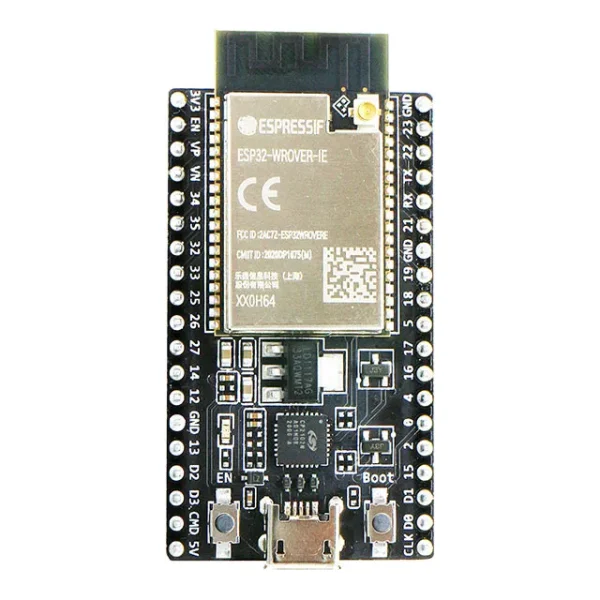
\includegraphics[width=\linewidth]{figures/esp32_devkitc}\\
    \scriptsize Example dev board (ESP32-DevKitC)
  \end{column}
\end{columns}
\end{frame}

\section[nosectionpage]{Peripherals \& I/O}
% --------------------------------------------------------------------
\begin{frame}{Peripherals \& I/O: Why Makers Love it}
\begin{columns}[T,onlytextwidth]
  \begin{column}{0.5\textwidth}
    \begin{itemize}
\item \textbf{GPIO-Matrix}: viele Pins können auf viele Funktionen geroutet werden
\item Analog: \textbf{12-bit ADC} (multiple channels), \textbf{DAC} (2 ch)
\item Serial buses: \textbf{UART}, \textbf{SPI}, \textbf{I\textsuperscript{2}C}, \textbf{I\textsuperscript{2}S}
\item Timing/Steuerung: Timer, Watchdogs, \textbf{PWM} (LED/Motor), \textbf{RMT}
\item Connectivity extras: \textbf{SD/SDIO}, \textbf{Ethernet MAC}, \textbf{TWAI (CAN)}
\item Human input: \textbf{capacitive touch} (on many ESP32 variants)
    \end{itemize}
    \footnotesize
    Practical note: pins are \textbf{3.3\,V only} (use level shifters for 5\,V sensors).
  \end{column}
  \begin{column}{0.5\textwidth}
    \centering
    % Download an ESP32 module photo and place it as: figures/esp32_module.jpg
    % Example page: https://www.espressif.com/sites/default/files/documentation/esp32_datasheet_en.pdf
    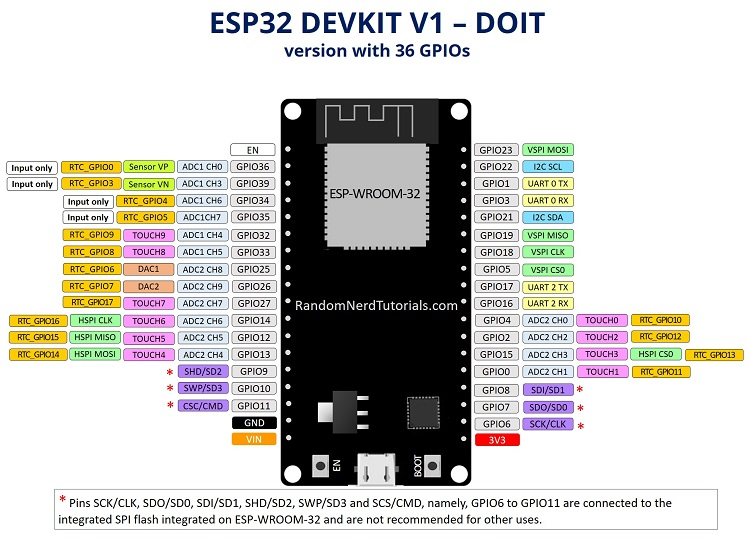
\includegraphics[width=\linewidth]{figures/ESP32-Pinout}\\
    \scriptsize ESP32 module (shield can + antenna)
  \end{column}
\end{columns}
\end{frame}

\section[nosectionpage]{Programming Ecosystem}
% --------------------------------------------------------------------
\begin{frame}{Programming Ecosystem (what students should remember)}
\begin{itemize}
\item \textbf{ESP-IDF (official)}: C/C++ toolchain, drivers, Wi-Fi/BLE stacks, FreeRTOS
\item \textbf{Arduino core}: easiest entry, huge library ecosystem
\item \textbf{MicroPython}: schnelles Prototyping, sehr gut für die Lehre
\item Typischer Ablauf: Code schreiben \(\rightarrow\) per USB flashen \(\rightarrow\) über Serial Monitor debuggen
\item Real-world concerns:
    \begin{itemize}
\item Power modes (deep-sleep), battery life
\item Wireless reliability (RSSI, antennas), OTA updates
\item Basic security: credentials, encrypted transport (TLS), secure boot options
    \end{itemize}
\end{itemize}
\vspace{0.3em}
\footnotesize
Mini-Demo-Idee: read a temperature sensor + publish via Wi-Fi (MQTT) or advertise via BLE.
\end{frame}